\section{Final Tables}
The summarized results are presented in three tables: 
\begin{itemize}
\item Table~\ref{tab:OSSF1tau0} contains observed yields  and background prediction 
for each search region in a tri-lepton channel with an opposite sign same flavour lepton pair present;
\item Table~\ref{tab:OSSF0tau0}  - for a channel without  an opposite sign same flavour lepton pair;
\item Table~\ref{tab:SStau1} - for a channel with a same sign di-lepton and a hadronically decaying tau (SS$\tau$);
\item Table~\ref{tab:OSOF1tau1} - for a channel with an opposite sign opposite flavour di-lepton and a hadronically decaying tau (OSOF$\tau$). This result is fully based on the Ref.~\cite{AN2012:255}.
\end{itemize}

The graphical representation of the results is shown in Figures~\ref{fig:OSSF1tau0},~\ref{fig:OSSF0tau0},~\ref{fig:SStau1},~\ref{fig:OSOF1tau1}.

%==========================================================================================
\begin{figure}[htp]
\begin{center}
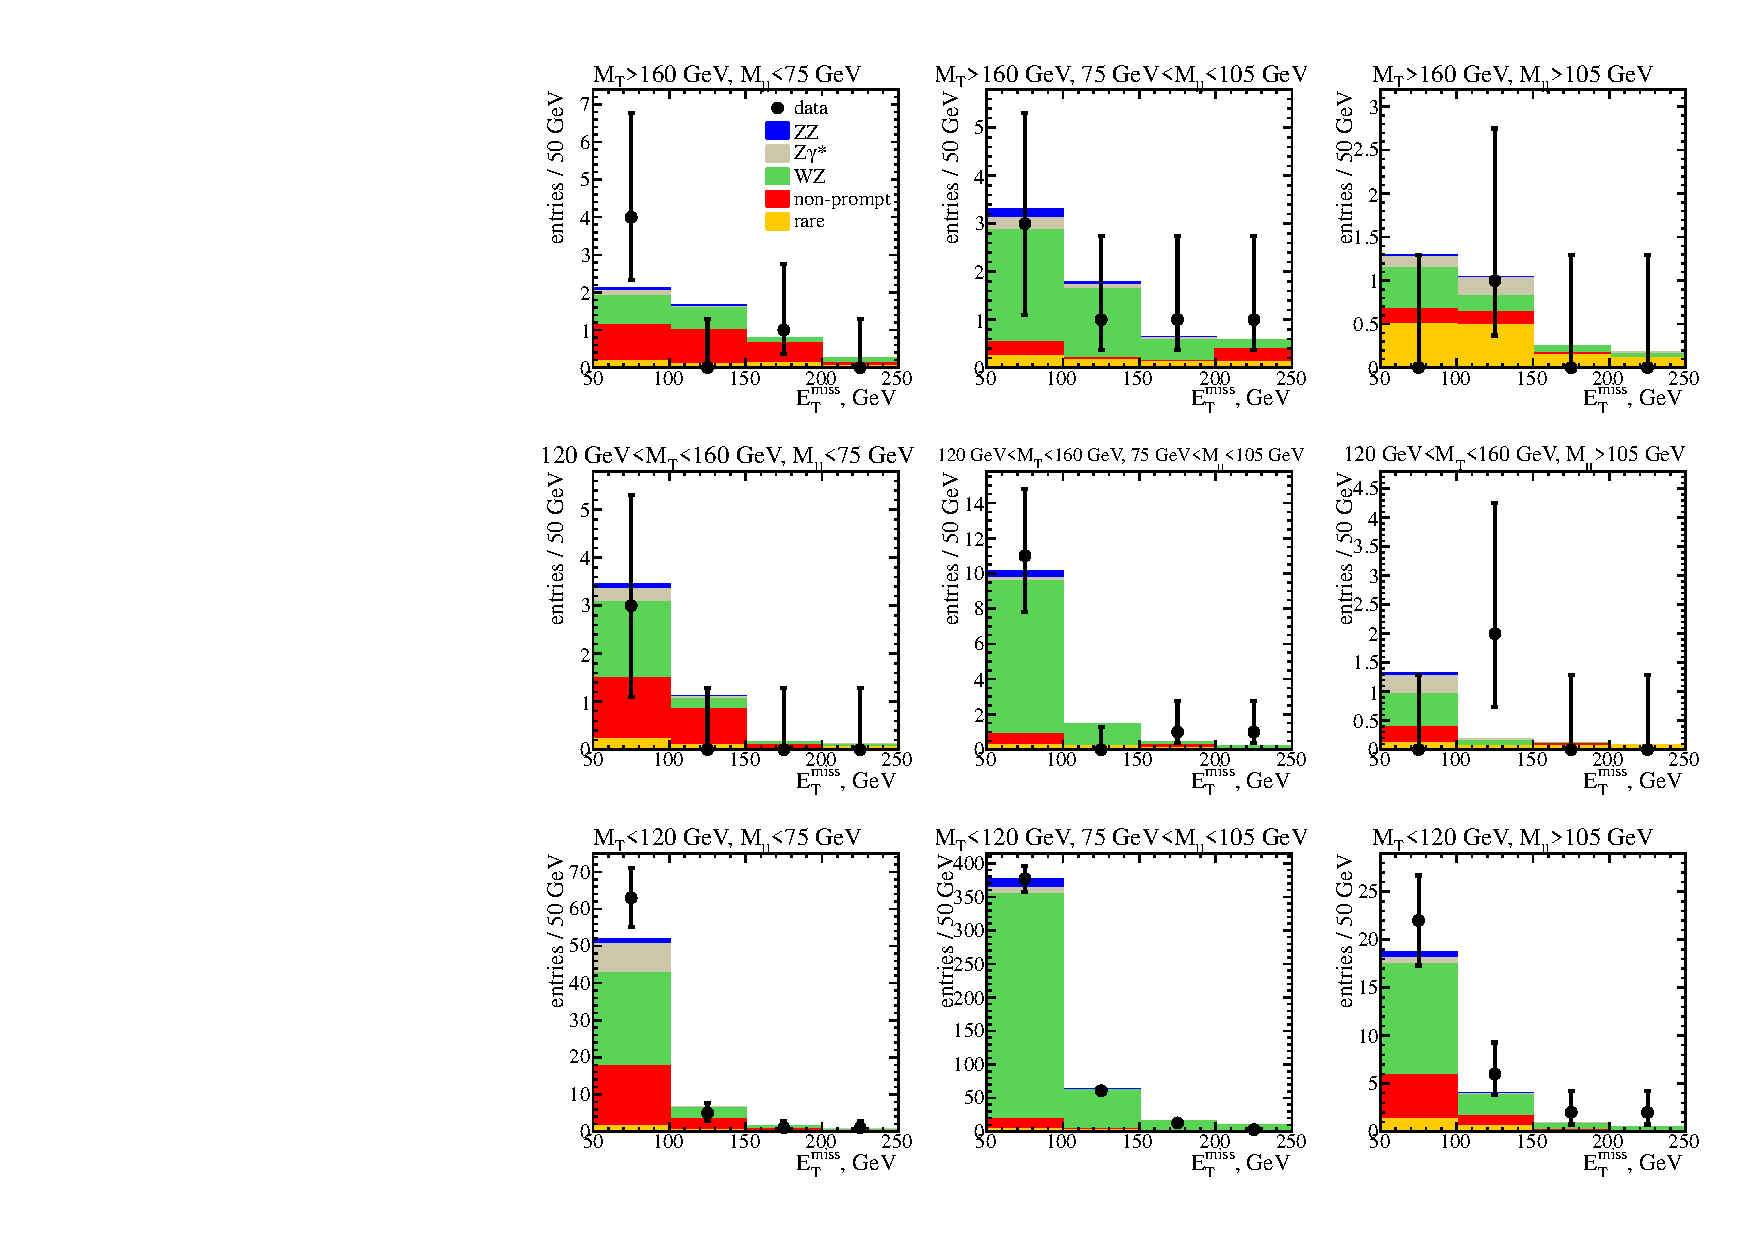
\includegraphics[width=1.0\textwidth]{plots/ossf1tau0.pdf}
\caption{Observed yields and predicted backgrounds for a tri-lepton with an opposite sign same flavour lepton pair present in all defined search regions.}
\label{fig:OSSF1tau0}
\end{center}
\end{figure}
%==========================================================================================

%==========================================================================================
\begin{figure}[htp]
\begin{center}
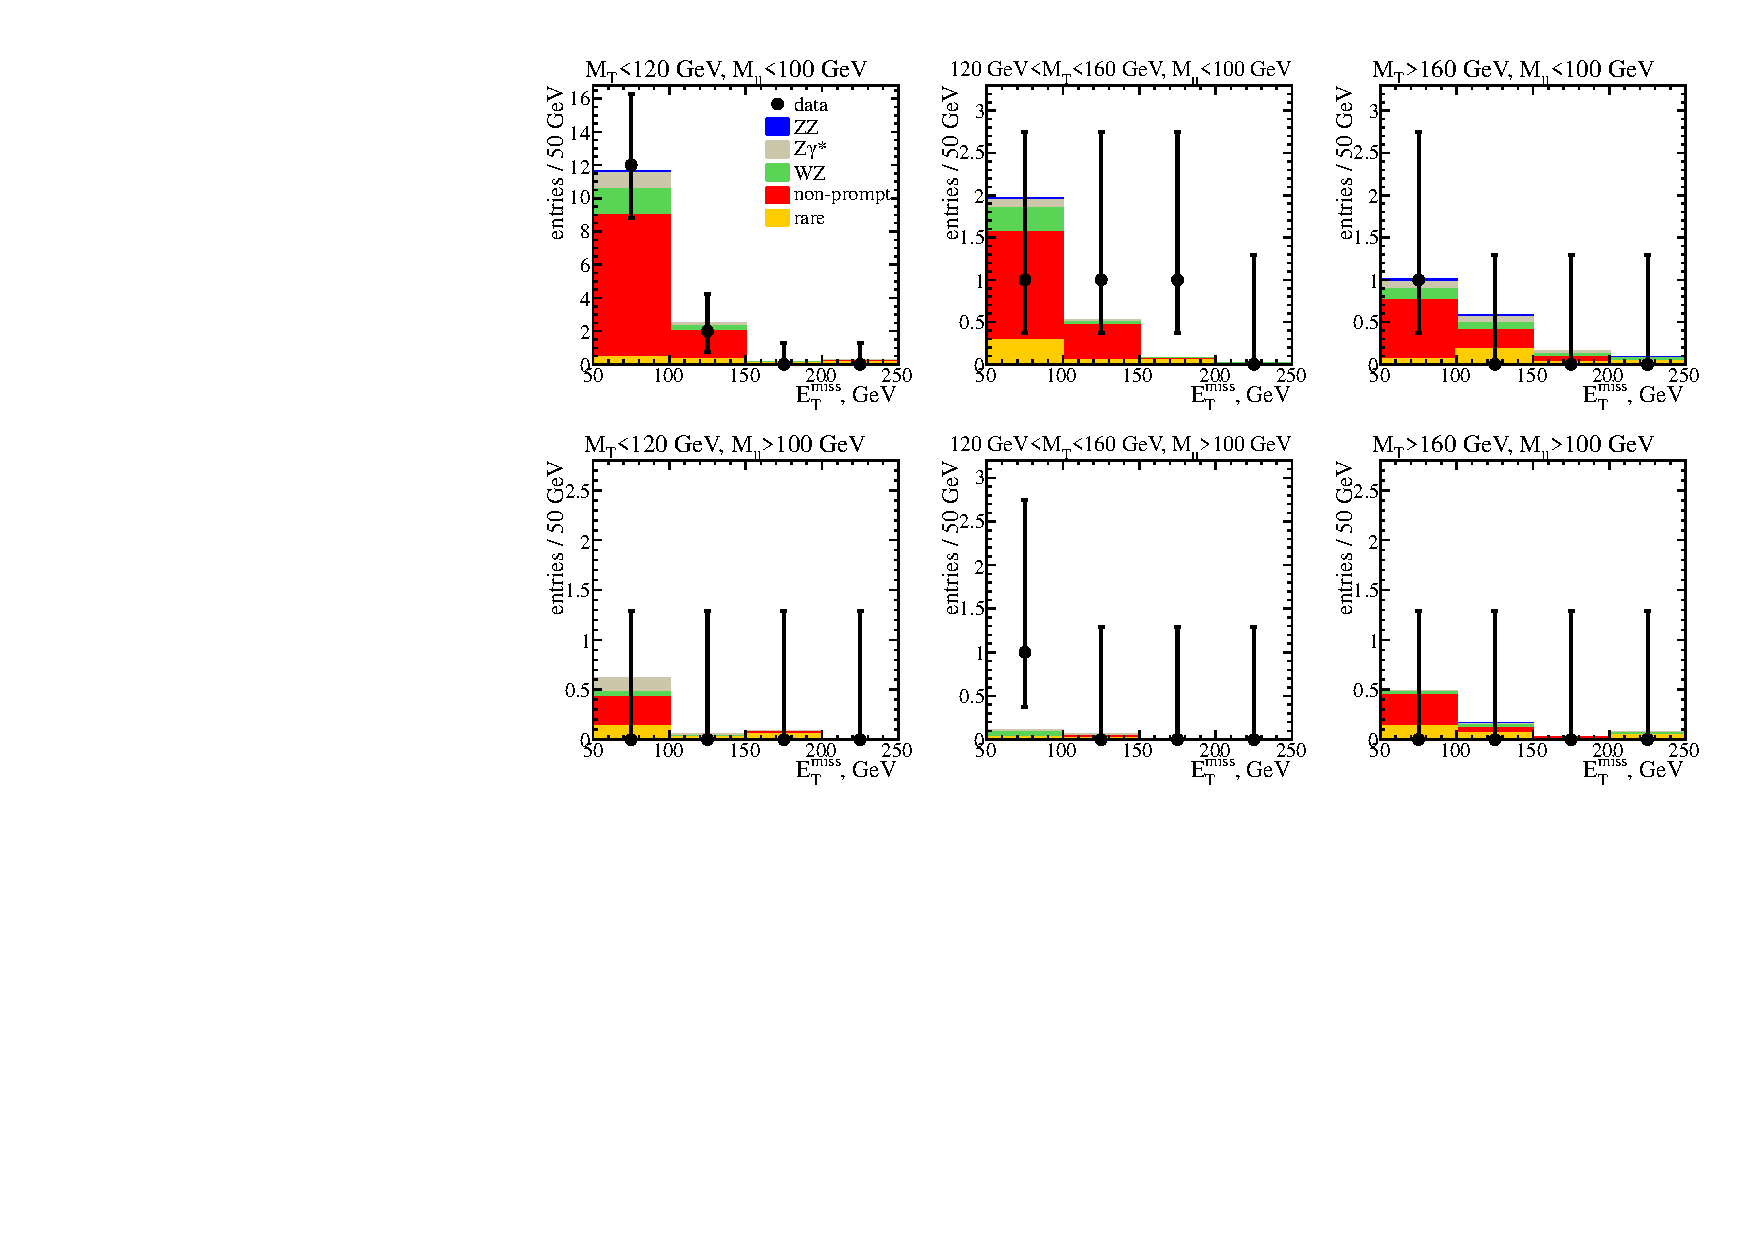
\includegraphics[width=1.0\textwidth]{plots/ossf0tau0.pdf}
\caption{Observed yields and predicted backgrounds for a tri-lepton without an opposite sign same flavour lepton pair present in all defined search regions.}
\label{fig:OSSF0tau0}
\end{center}
\end{figure}
%==========================================================================================

%==========================================================================================
\begin{figure}[htp]
\begin{center}
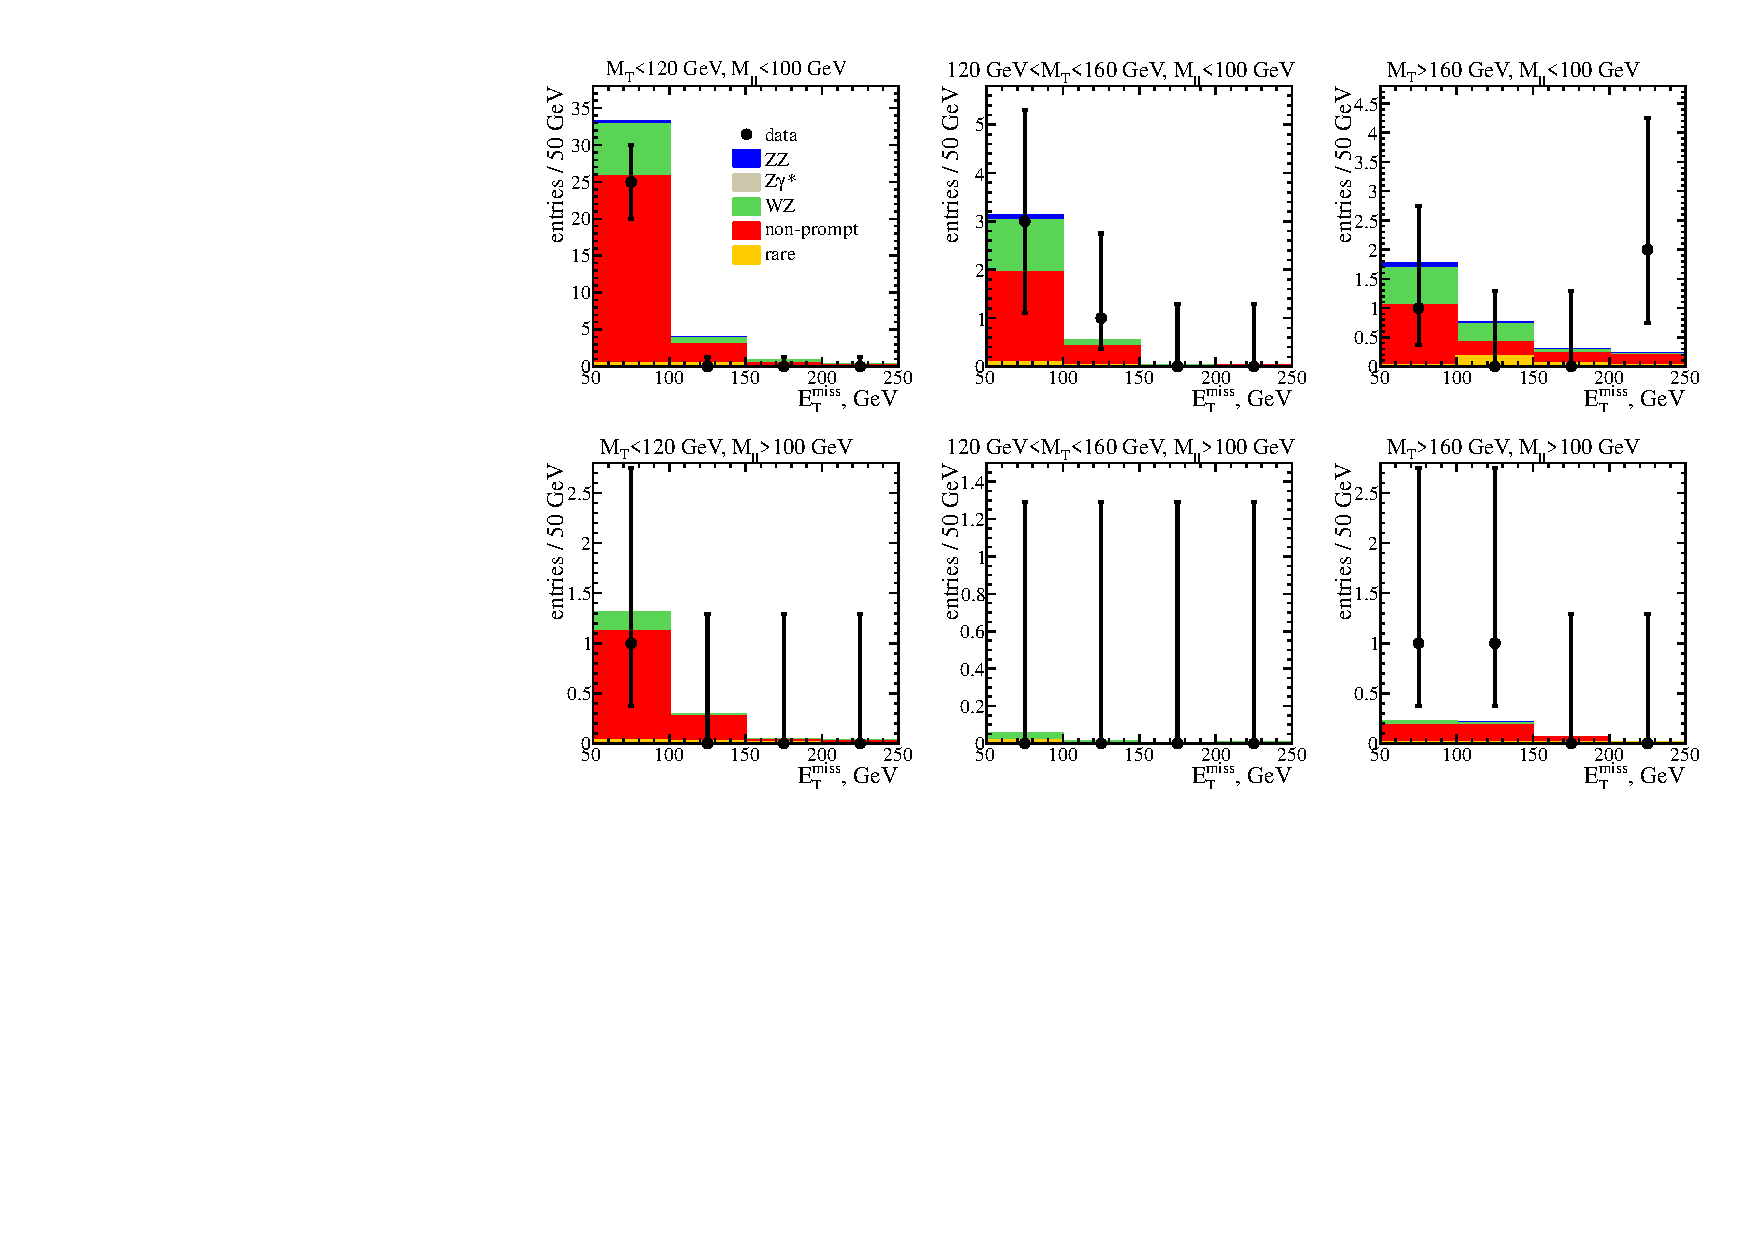
\includegraphics[width=1.0\textwidth]{plots/ossf0tau1.pdf}
\caption{Observed yields and predicted backgrounds for a tri-lepton with a same sign di-lepton and a hadronically decaying tau in all defined search regions.}
\label{fig:SStau1}
\end{center}
\end{figure}
%==========================================================================================

%==========================================================================================
\begin{figure}[htp]
\begin{center}
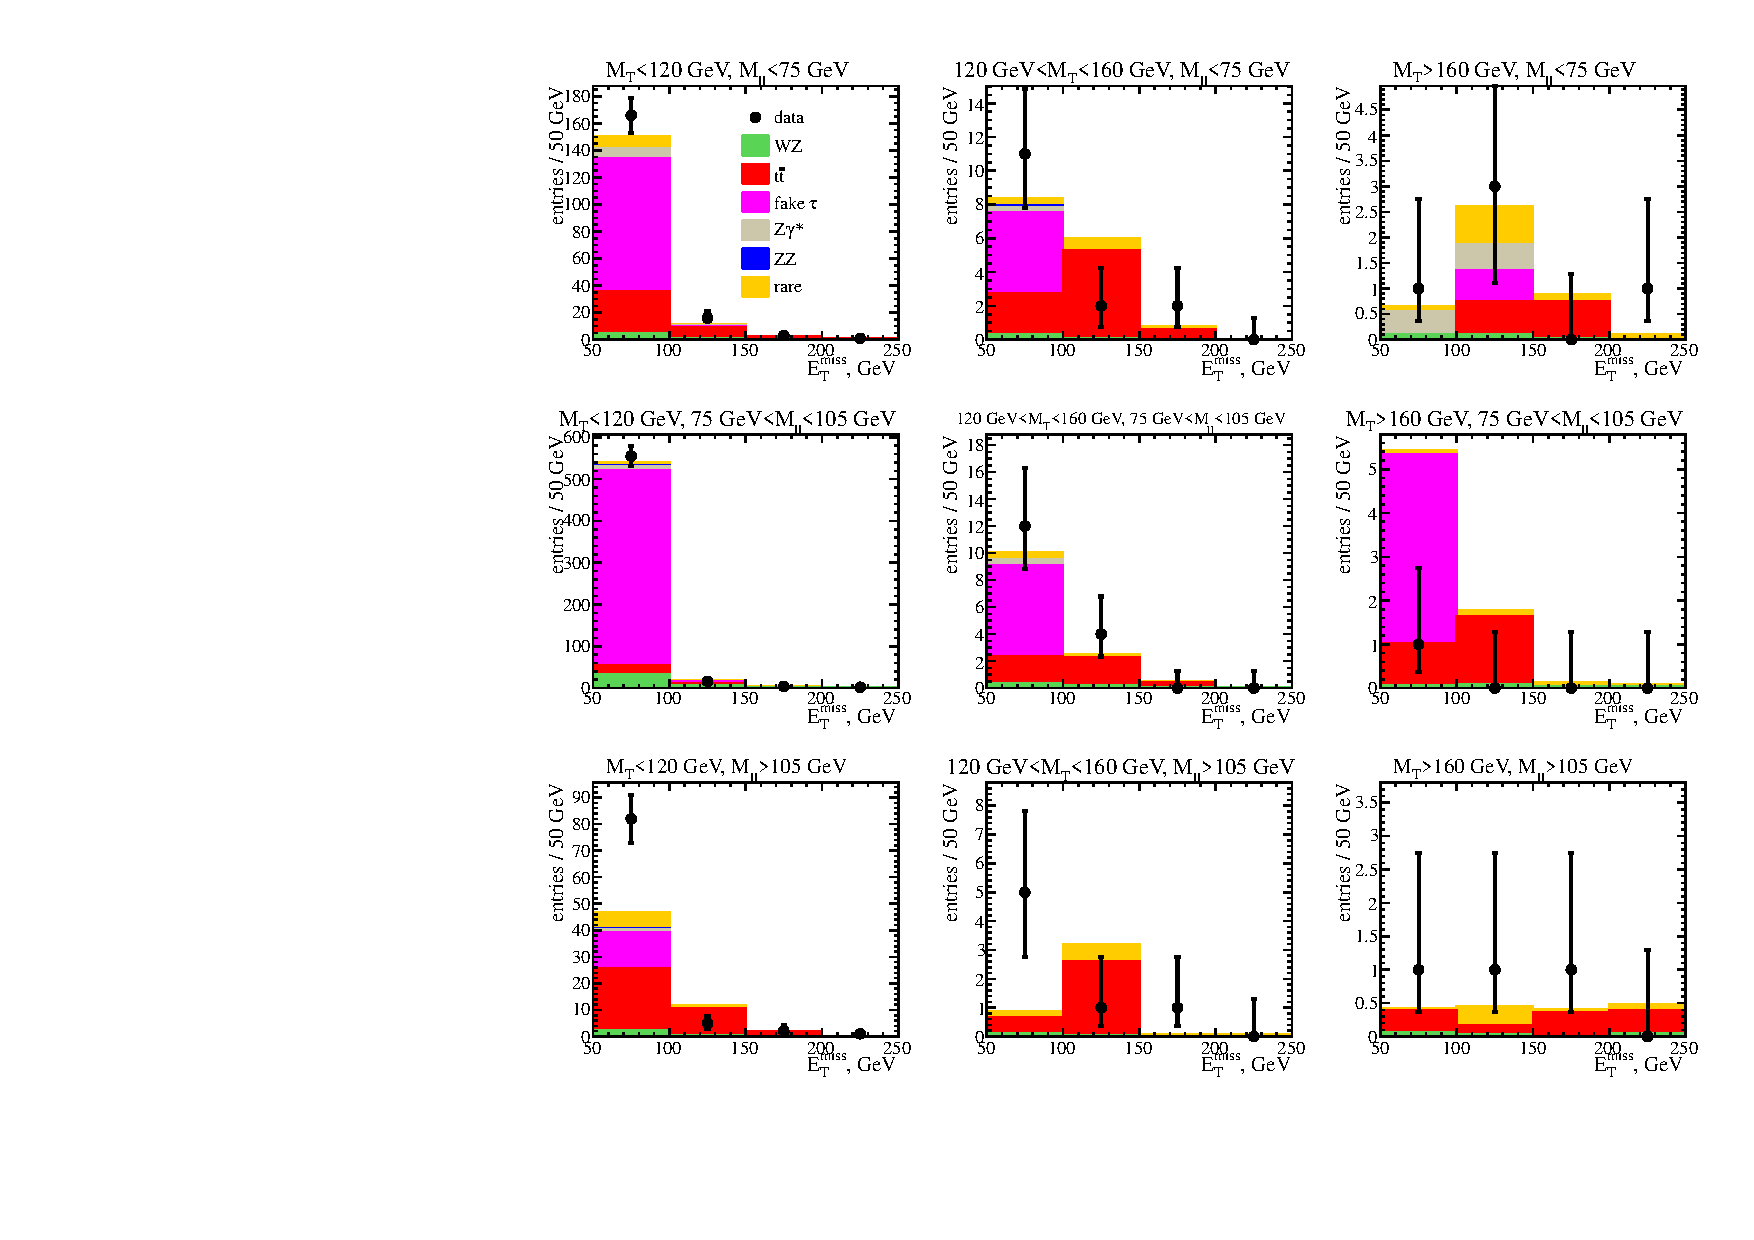
\includegraphics[width=1.0\textwidth]{plots/osof1tau1.pdf}
\caption{Observed yields and predicted backgrounds for a tri-lepton with an opposite sign opposite flavour di-lepton and a hadronically decaying tau  in all defined search regions.}
\label{fig:OSOF1tau1}
\end{center}
\end{figure}
%==========================================================================================

\begin{landscape}
%==========================================================================================
%==========================================================================================
\begin{table}
\begin{center}
\caption{\label{tab:OSSF1tau0} The summary of the observed yields and predicted backgrounds for tri-lepton with opposite sign same flavour pair present. }
\begin{tabular}{| c | c c c c c c c | }\hline\hline
$\ETmiss$ (GeV) & WZ & Non-Prompt & Rare SM & Z$\gamma^*$ & ZZ & Total bkg & Observed\\\hline\hline
\multicolumn{7}{l}{$M_{\text{T}} < 120$ GeV, $M_{\ell\ell} < 75$ GeV}\\\hline\hline
50$\dots$100&26$\pm$2.7&17$\pm$3.3&1.4$\pm$0.84&6.8$\pm$0.3&1.3$\pm$0.072&52$\pm$4.4&63\\
100$\dots$150&3.4$\pm$0.42&3.9$\pm$0.85&0.42$\pm$0.24&0.097$\pm$0.041&0.11$\pm$0.022&8$\pm$0.98&5\\
150$\dots$200&0.99$\pm$0.19&0.61$\pm$0.19&0.19$\pm$0.13&0.021$\pm$0.017&0.011$\pm$0.006&1.8$\pm$0.3&1\\
200$\dots$250&0.4$\pm$0.082&0.19$\pm$0.075&0.082$\pm$0.058&0.043$\pm$0.016&0.014$\pm$0.007&0.74$\pm$0.13&1\\
\hline\hline
\multicolumn{7}{l}{$120~\mathrm{GeV} < M_{\text{T}} < 160~\mathrm{GeV}$, $M_{\ell\ell} < 75$ GeV}\\\hline\hline
50$\dots$100&1.6$\pm$0.22&0.97$\pm$0.38&0.22$\pm$0.14&0.23$\pm$0.054&0.11$\pm$0.022&3.1$\pm$0.47&3\\
100$\dots$150&0.24$\pm$0.038&0.61$\pm$0.3&0.091$\pm$0.067&0.043$\pm$0.023&0.0051$\pm$0.0051&0.99$\pm$0.31&0\\
150$\dots$200&0.063$\pm$0.017&0.08$\pm$0.052&0.0046$\pm$0.0052&0$\pm$0.00049&0$\pm$0&0.15$\pm$0.055&0\\
200$\dots$250&0.043$\pm$0.015&0.075$\pm$0.037&0.044$\pm$0.044&0.022$\pm$0.018&0$\pm$0&0.18$\pm$0.062&0\\
\hline\hline
\multicolumn{7}{l}{$M_{\text{T}} > 160$ GeV, $M_{\ell\ell} < 75$ GeV}\\\hline\hline
50$\dots$100&0.8$\pm$0.28&0.77$\pm$0.47&0.16$\pm$0.19&0.13$\pm$0.04&0.096$\pm$0.021&1.9$\pm$0.58&4\\
100$\dots$150&0.6$\pm$0.21&0.75$\pm$0.54&0.096$\pm$0.11&0.022$\pm$0.016&0.058$\pm$0.015&1.5$\pm$0.59&0\\
150$\dots$200&0.16$\pm$0.063&0.61$\pm$0.48&0.11$\pm$0.13&0$\pm$0.0049&0.019$\pm$0.0093&0.9$\pm$0.5&1\\
200$\dots$250&0.18$\pm$0.07&0.064$\pm$0.042&0.033$\pm$0.038&0$\pm$0.0002&0.012$\pm$0.0048&0.28$\pm$0.09&0\\
\hline\hline
\multicolumn{7}{l}{$M_{\text{T}} < 120$ GeV, $75~\mathrm{GeV} < M_{\ell\ell} < 105~\mathrm{GeV}$}\\\hline\hline
50$\dots$100&333$\pm$33&22.6$\pm$3.7&4.1$\pm$2.2&8.2$\pm$0.3&13.1$\pm$0.2&381$\pm$33&377\\
100$\dots$150&59$\pm$6.2&2.6$\pm$0.69&1.8$\pm$1&0.14$\pm$0.049&1.6$\pm$0.083&65$\pm$6.3&61\\
150$\dots$200&15$\pm$1.9&0.49$\pm$0.14&0.64$\pm$0.35&0.022$\pm$0.019&0.29$\pm$0.035&17$\pm$1.9&13\\
200$\dots$250&8.9$\pm$1.2&0.12$\pm$0.029&0.55$\pm$0.3&0.043$\pm$0.00092&0.13$\pm$0.018&9.8$\pm$1.2&3\\
\hline\hline
\multicolumn{7}{l}{$120~\mathrm{GeV} < M_{\text{T}} < 160~\mathrm{GeV}$, $75~\mathrm{GeV} < M_{\ell\ell} < 105~\mathrm{GeV}$}\\\hline\hline
50$\dots$100&8.4$\pm$1.1&0.6$\pm$0.35&0.25$\pm$0.15&0.15$\pm$0.043&0.43$\pm$0.042&9.8$\pm$1.2&11\\
100$\dots$150&1.2$\pm$0.17&0.042$\pm$0.029&0.17$\pm$0.11&0$\pm$0.0053&0.044$\pm$0.014&1.5$\pm$0.21&0\\
150$\dots$200&0.18$\pm$0.043&0.046$\pm$0.031&0.071$\pm$0.054&0$\pm$0.00027&0$\pm$0&0.3$\pm$0.075&1\\
200$\dots$250&0.12$\pm$0.025&0.029$\pm$0.031&0.014$\pm$0.014&0$\pm$0.00025&0$\pm$0&0.17$\pm$0.042&1\\
\hline\hline
\end{tabular}
\end{center}
\end{table}
%==========================================================================================
%==========================================================================================
\begin{table*}
\begin{center}
%\caption{Continuation}
\begin{tabular}{| c | c c c c c c c | }\hline\hline
$\ETmiss$ (GeV) & WZ & Non-Prompt & Rare SM & Z$\gamma^*$ & ZZ & Total bkg & Observed\\\hline\hline
\multicolumn{7}{l}{$M_{\text{T}} > 160$ GeV, $75~\mathrm{GeV} < M_{\ell\ell} < 105~\mathrm{GeV}$}\\\hline\hline
50$\dots$100&2.3$\pm$0.72&0.34$\pm$0.14&0.24$\pm$0.27&0.24$\pm$0.054&0.17$\pm$0.026&3.2$\pm$0.78&3\\
100$\dots$150&1.5$\pm$0.49&0.078$\pm$0.047&0.15$\pm$0.17&0.065$\pm$0.028&0.036$\pm$0.013&1.8$\pm$0.53&1\\
150$\dots$200&0.48$\pm$0.17&0.015$\pm$0.016&0.12$\pm$0.14&0.043$\pm$0.023&0.015$\pm$0.0081&0.67$\pm$0.22&1\\
200$\dots$250&0.22$\pm$0.089&0.37$\pm$0.33&0.11$\pm$0.13&0$\pm$0.0001&0.01$\pm$0.0073&0.71$\pm$0.36&1\\
\hline\hline
\multicolumn{7}{l}{$M_{\text{T}} < 120$ GeV, $M_{\ell\ell} > 105$ GeV}\\\hline\hline
50$\dots$100&12$\pm$1.2&5.4$\pm$1.1&1.2$\pm$0.7&0.73$\pm$0.11&0.6$\pm$0.052&19$\pm$1.8&22\\
100$\dots$150&2.3$\pm$0.25&1.3$\pm$0.35&0.53$\pm$0.3&0.12$\pm$0.046&0.13$\pm$0.024&4.4$\pm$0.53&6\\
150$\dots$200&0.62$\pm$0.087&0.24$\pm$0.078&0.078$\pm$0.047&0.03$\pm$0.026&0.011$\pm$0.0053&0.98$\pm$0.13&2\\
200$\dots$250&0.37$\pm$0.053&0.028$\pm$0.018&0.029$\pm$0.021&0$\pm$0.00051&0.024$\pm$0.0078&0.45$\pm$0.06&2\\
\hline\hline
\multicolumn{7}{l}{$120~\mathrm{GeV} < M_{\text{T}} < 160~\mathrm{GeV}$, $M_{\ell\ell} > 105$ GeV}\\\hline\hline
50$\dots$100&0.6$\pm$0.086&0.68$\pm$0.4&0.11$\pm$0.071&0.27$\pm$0.058&0.033$\pm$0.012&1.7$\pm$0.42&0\\
100$\dots$150&0.091$\pm$0.021&0.18$\pm$0.088&0.055$\pm$0.047&0.021$\pm$0.017&0$\pm$0&0.35$\pm$0.1&2\\
150$\dots$200&0.033$\pm$0.01&0.052$\pm$0.033&0.055$\pm$0.049&0$\pm$0.0047&0$\pm$0&0.14$\pm$0.06&0\\
200$\dots$250&0.0019$\pm$0.0023&0.027$\pm$0.019&0.077$\pm$0.086&0$\pm$0.00017&0$\pm$0&0.11$\pm$0.088&0\\
\hline\hline
\multicolumn{7}{l}{$M_{\text{T}} > 160$ GeV, $M_{\ell\ell} > 105$ GeV}\\\hline\hline
50$\dots$100&0.46$\pm$0.16&0.38$\pm$0.19&0.5$\pm$0.66&0.14$\pm$0.045&0.0089$\pm$0.0053&1.5$\pm$0.71&0\\
100$\dots$150&0.21$\pm$0.081&0.22$\pm$0.059&0.49$\pm$0.62&0.19$\pm$0.05&0.014$\pm$0.0078&1.1$\pm$0.63&1\\
150$\dots$200&0.084$\pm$0.032&0.13$\pm$0.043&0.14$\pm$0.17&0$\pm$0.01&0.00068$\pm$0.00068&0.35$\pm$0.18&0\\
200$\dots$250&0.056$\pm$0.022&0.0037$\pm$8.8e-05&0.11$\pm$0.14&0.021$\pm$0.00029&0.0027$\pm$0.0027&0.19$\pm$0.14&0\\
\hline\hline
\end{tabular}
\end{center}
\end{table*}
%==========================================================================================
%==========================================================================================
\begin{table}
\small
\begin{center}
\caption{\label{tab:OSSF0tau0} The summary of the observed yields and predicted backgrounds for tri-lepton without opposite sign same flavour pair present. }
\begin{tabular}{| c | c c c c c c c | }\hline\hline
$\ETmiss$ (GeV) & WZ & Non-Prompt & Rare SM & Z$\gamma^*$ & ZZ & Total bkg & Observed\\\hline\hline
\multicolumn{7}{l}{$M_{\text{T}} < 120$ GeV, $M_{\ell\ell} < 75$ GeV}\\\hline\hline
50$\dots$100&1.6$\pm$0.16&9.4$\pm$2.1&0.44$\pm$0.26&0.92$\pm$0.092&0.13$\pm$0.023&12$\pm$2.1&12\\
100$\dots$150&0.32$\pm$0.053&2.1$\pm$0.48&0.29$\pm$0.18&0.21$\pm$0.04&0.019$\pm$0.0089&2.9$\pm$0.52&2\\
150$\dots$200&0.085$\pm$0.026&0.37$\pm$0.12&0.062$\pm$0.05&0.024$\pm$0.015&0$\pm$0&0.54$\pm$0.13&0\\
200$\dots$250&0.029$\pm$0.0081&0.099$\pm$0.026&0.13$\pm$0.14&0.032$\pm$0.015&0$\pm$0&0.29$\pm$0.14&0\\
\hline\hline
\multicolumn{7}{l}{$120~\mathrm{GeV} < M_{\text{T}} < 160~\mathrm{GeV}$, $M_{\ell\ell} < 75$ GeV}\\\hline\hline
50$\dots$100&0.29$\pm$0.042&1.3$\pm$0.43&0.28$\pm$0.22&0.1$\pm$0.029&0.027$\pm$0.011&2$\pm$0.49&1\\
100$\dots$150&0.029$\pm$0.011&0.33$\pm$0.096&0.051$\pm$0.036&0.032$\pm$0.015&0.0045$\pm$0.0045&0.45$\pm$0.1&1\\
150$\dots$200&0.019$\pm$0.0084&0.074$\pm$0.03&0.047$\pm$0.046&0$\pm$0.005&0$\pm$0&0.14$\pm$0.055&1\\
200$\dots$250&0.003$\pm$0.0038&0.058$\pm$0.038&0.0068$\pm$0.0062&0$\pm$0&0$\pm$0&0.068$\pm$0.039&0\\
\hline\hline
\multicolumn{7}{l}{$M_{\text{T}} > 160$ GeV, $M_{\ell\ell} < 75$ GeV}\\\hline\hline
50$\dots$100&0.14$\pm$0.051&0.63$\pm$0.26&0.058$\pm$0.068&0.095$\pm$0.026&0.017$\pm$0.009&0.95$\pm$0.28&1\\
100$\dots$150&0.11$\pm$0.044&0.87$\pm$0.35&0.18$\pm$0.23&0.079$\pm$0.024&0.028$\pm$0.012&1.3$\pm$0.42&0\\
150$\dots$200&0.033$\pm$0.014&0.094$\pm$0.037&0.022$\pm$0.026&0.025$\pm$0.012&0.002$\pm$0.002&0.18$\pm$0.049&0\\
200$\dots$250&0.04$\pm$0.019&0.057$\pm$0.025&0.039$\pm$0.047&0$\pm$0.00014&0.0028$\pm$0.00063&0.14$\pm$0.057&0\\
\hline\hline
\multicolumn{7}{l}{$M_{\text{T}} < 120$ GeV, $M_{\ell\ell} > 105$ GeV}\\\hline\hline
50$\dots$100&0.041$\pm$0.012&0.53$\pm$0.15&0.14$\pm$0.086&0.18$\pm$0.035&0$\pm$0&0.88$\pm$0.18&0\\
100$\dots$150&0.0064$\pm$0.0037&0.17$\pm$0.039&0.025$\pm$0.019&0.032$\pm$0.016&0$\pm$0&0.24$\pm$0.046&0\\
150$\dots$200&0$\pm$0&0.065$\pm$0.028&0.056$\pm$0.049&0.011$\pm$0.0084&0$\pm$0&0.13$\pm$0.057&0\\
200$\dots$250&0$\pm$0&0.02$\pm$0.012&0.00021$\pm$0.00017&0$\pm$0.0043&0$\pm$0&0.02$\pm$0.013&0\\
\hline\hline
\multicolumn{7}{l}{$120~\mathrm{GeV} < M_{\text{T}} < 160~\mathrm{GeV}$, $M_{\ell\ell} > 105$ GeV}\\\hline\hline
50$\dots$100&0.057$\pm$0.013&0.002$\pm$0.0015&0.023$\pm$0.019&0.021$\pm$0.011&0$\pm$0&0.1$\pm$0.025&1\\
100$\dots$150&0.0037$\pm$0.0036&0.0023$\pm$0.0016&0.014$\pm$0.014&0.022$\pm$0.011&0$\pm$0&0.042$\pm$0.018&0\\
150$\dots$200&0$\pm$0&0$\pm$0&0.00021$\pm$0.00018&0$\pm$3.4e-05&0$\pm$0&0.00021$\pm$0.00019&0\\
200$\dots$250&0$\pm$0&0$\pm$3.5e-05&0.004$\pm$0.0046&0$\pm$2.8e-05&0$\pm$0&0.004$\pm$0.0046&0\\
\hline\hline
\multicolumn{7}{l}{$M_{\text{T}} > 160$ GeV, $M_{\ell\ell} > 105$ GeV}\\\hline\hline
50$\dots$100&0.022$\pm$0.011&0.19$\pm$0.18&0.13$\pm$0.16&0.022$\pm$0.012&0.00079$\pm$0.00079&0.37$\pm$0.24&0\\
100$\dots$150&0.026$\pm$0.012&0.11$\pm$0.046&0.06$\pm$0.076&0.022$\pm$0.013&0.0044$\pm$0.0044&0.22$\pm$0.091&0\\
150$\dots$200&0.0033$\pm$0.0031&0.021$\pm$0.022&0.00061$\pm$0.00073&0$\pm$0.00011&0.0044$\pm$0.0044&0.03$\pm$0.023&0\\
200$\dots$250&0.021$\pm$0.0099&0$\pm$6.7e-05&0.044$\pm$0.058&0.011$\pm$0.0081&0$\pm$0&0.075$\pm$0.059&0\\
\hline\hline
\end{tabular}
\end{center}
\end{table}
%==========================================================================================
%==========================================================================================
\begin{table}
\small
\begin{center}
\caption{\label{tab:SStau1} The summary of the observed yields and predicted backgrounds for the channel with a same sign di-lepton and a hadronically decaying tau. }
\begin{tabular}{| c | c c c c c c c | }\hline\hline
$\ETmiss$ (GeV) & WZ & Non-Prompt & Rare SM & Z$\gamma^*$ & ZZ & Total bkg & Observed\\\hline\hline
\multicolumn{7}{l}{$M_{\text{T}} < 120$ GeV, $M_{\ell\ell} < 75$ GeV}\\\hline\hline
50$\dots$100&7.1$\pm$0.18&25$\pm$4.6&0.42$\pm$0.23&0$\pm$0&0.41$\pm$0.041&33$\pm$4.6&25\\
100$\dots$150&0.87$\pm$0.065&2.6$\pm$0.68&0.4$\pm$0.4&0$\pm$0&0.022$\pm$0.0097&3.9$\pm$0.79&0\\
150$\dots$200&0.4$\pm$0.044&0.39$\pm$0.19&0.032$\pm$0.027&0$\pm$0&0.0088$\pm$0.0059&0.83$\pm$0.2&0\\
200$\dots$250&0.21$\pm$0.032&0.071$\pm$0.056&0.023$\pm$0.017&0$\pm$0&0.0056$\pm$0.00069&0.31$\pm$0.067&0\\
\hline\hline
\multicolumn{7}{l}{$120~\mathrm{GeV} < M_{\text{T}} < 160~\mathrm{GeV}$, $M_{\ell\ell} < 75$ GeV}\\\hline\hline
50$\dots$100&1.1$\pm$0.072&1.9$\pm$0.55&0.078$\pm$0.059&0$\pm$0&0.095$\pm$0.02&3.1$\pm$0.56&3\\
100$\dots$150&0.12$\pm$0.024&0.39$\pm$0.19&0.027$\pm$0.024&0$\pm$0&0.0061$\pm$0.0044&0.54$\pm$0.2&1\\
150$\dots$200&0.02$\pm$0.0097&0$\pm$0&0.0084$\pm$0.0098&0$\pm$0&0$\pm$0&0.028$\pm$0.014&0\\
200$\dots$250&0.0054$\pm$0.0051&0.022$\pm$0.023&0.0035$\pm$0.0035&0$\pm$0&0$\pm$0&0.031$\pm$0.024&0\\
\hline\hline
\multicolumn{7}{l}{$M_{\text{T}} > 160$ GeV, $M_{\ell\ell} < 75$ GeV}\\\hline\hline
50$\dots$100&0.62$\pm$0.055&1$\pm$0.37&0.028$\pm$0.023&0$\pm$0&0.12$\pm$0.023&1.8$\pm$0.37&1\\
100$\dots$150&0.3$\pm$0.038&0.25$\pm$0.14&0.17$\pm$0.14&0$\pm$0&0.046$\pm$0.014&0.76$\pm$0.2&0\\
150$\dots$200&0.061$\pm$0.017&0.17$\pm$0.15&0.054$\pm$0.041&0$\pm$0&0.0078$\pm$0.006&0.29$\pm$0.16&0\\
200$\dots$250&0.03$\pm$0.012&0.16$\pm$0.12&0.028$\pm$0.024&0$\pm$0&0.01$\pm$0.0062&0.23$\pm$0.12&2\\
\hline\hline
\multicolumn{7}{l}{$M_{\text{T}} < 120$ GeV, $M_{\ell\ell} > 105$ GeV}\\\hline\hline
50$\dots$100&0.19$\pm$0.03&1.1$\pm$0.4&0.035$\pm$0.029&0$\pm$0&0.0074$\pm$0.0058&1.3$\pm$0.41&1\\
100$\dots$150&0.025$\pm$0.011&0.25$\pm$0.11&0.02$\pm$0.019&0$\pm$0&0$\pm$0&0.29$\pm$0.11&0\\
150$\dots$200&0.011$\pm$0.0073&0.022$\pm$0.023&0.0083$\pm$0.0082&0$\pm$0&0$\pm$0&0.042$\pm$0.026&0\\
200$\dots$250&0.0047$\pm$0.0048&0.022$\pm$0.023&0.00011$\pm$0.00011&0$\pm$0&0$\pm$0&0.027$\pm$0.024&0\\
\hline\hline
\multicolumn{7}{l}{$120~\mathrm{GeV} < M_{\text{T}} < 160~\mathrm{GeV}$, $M_{\ell\ell} > 105$ GeV}\\\hline\hline
50$\dots$100&0.035$\pm$0.013&0$\pm$0&0.02$\pm$0.018&0$\pm$0&0$\pm$0&0.055$\pm$0.023&0\\
100$\dots$150&0.013$\pm$0.0079&0$\pm$0&0.00015$\pm$0.00014&0$\pm$0&0$\pm$0&0.013$\pm$0.0079&0\\
150$\dots$200&0$\pm$0&0$\pm$0&0$\pm$0&0$\pm$0&0$\pm$0&0$\pm$0&0\\
200$\dots$250&0.0065$\pm$0.0056&0$\pm$0&0$\pm$0&0$\pm$0&0$\pm$0&0.0065$\pm$0.0056&0\\
\hline\hline
\multicolumn{7}{l}{$M_{\text{T}} > 160$ GeV, $M_{\ell\ell} > 105$ GeV}\\\hline\hline
50$\dots$100&0.034$\pm$0.013&0.18$\pm$0.12&0.0079$\pm$0.0066&0$\pm$0&0$\pm$0&0.22$\pm$0.13&1\\
100$\dots$150&0.025$\pm$0.011&0.17$\pm$0.15&0.0093$\pm$0.0086&0$\pm$0&0.0019$\pm$0.0019&0.21$\pm$0.15&1\\
150$\dots$200&0$\pm$0&0.053$\pm$0.041&0.012$\pm$0.013&0$\pm$0&0$\pm$0&0.065$\pm$0.043&0\\
200$\dots$250&0$\pm$0&0$\pm$0&0.011$\pm$0.0085&0$\pm$0&0$\pm$0&0.011$\pm$0.0085&0\\
\hline\hline
\end{tabular}
\end{center}
\end{table}
%==========================================================================================
%==========================================================================================
\begin{table}
\begin{center}
\caption{\label{tab:OSOF1tau1} The summary of the observed yields and predicted backgrounds for the channel with an OSOF di-lepton and a hadronically decaying tau. }
\begin{tabular}{| c | c c c c c c  | c  c | }\hline\hline
$\ETmiss$ (GeV) & WZ & $t\bar{t}$ & Fake tau & Z$\gamma^*$ & ZZ & Rare SM & Total bkg & Observed\\\hline\hline
\multicolumn{7}{l}{$M_{\text{T}} < 120$ GeV, $M_{\ell\ell} < 75$ GeV}\\\hline\hline
50$\dots$100&4.5$\pm$1.3&31$\pm$17&99$\pm$49&7.4$\pm$3.5&0.56$\pm$0.35&8.8$\pm$4.8&151$\pm$58&166\\
100$\dots$150&0.76$\pm$0.23&8.1$\pm$4.7&0.92$\pm$0.82&0.44$\pm$0.48&0$\pm$0&1.4$\pm$0.76&12$\pm$5.2&16\\
150$\dots$200&0.23$\pm$0.075&2.4$\pm$1.6&0$\pm$0&0$\pm$0&0$\pm$0&0.068$\pm$0.052&2.7$\pm$1.6&3\\
200$\dots$250&0.098$\pm$0.038&0.77$\pm$0.62&0$\pm$0&0$\pm$0&0$\pm$0&0.031$\pm$0.027&0.9$\pm$0.63&1\\
\hline\hline
\multicolumn{7}{l}{$120~\mathrm{GeV} < M_{\text{T}} < 160~\mathrm{GeV}$, $M_{\ell\ell} < 75$ GeV}\\\hline\hline
50$\dots$100&0.31$\pm$0.12&2.4$\pm$1.7&4.8$\pm$3.3&0.31$\pm$0.36&0.085$\pm$0.098&0.43$\pm$0.28&8.4$\pm$4.3&11\\
100$\dots$150&0.062$\pm$0.029&5.2$\pm$3.4&0$\pm$0&0$\pm$0&0$\pm$0&0.71$\pm$0.55&6$\pm$3.5&2\\
150$\dots$200&0.043$\pm$0.024&0.6$\pm$0.55&0$\pm$0&0$\pm$0&0$\pm$0&0.15$\pm$0.12&0.79$\pm$0.58&2\\
200$\dots$250&0.0057$\pm$0.006&0$\pm$0&0$\pm$0&0$\pm$0&0$\pm$0&0.022$\pm$0.024&0.027$\pm$0.025&0\\
\hline\hline
\multicolumn{7}{l}{$M_{\text{T}} > 160$ GeV, $M_{\ell\ell} < 75$ GeV}\\\hline\hline
50$\dots$100&0.11$\pm$0.12&0$\pm$0&0$\pm$0&0.44$\pm$0.65&0$\pm$0&0.089$\pm$0.11&0.64$\pm$0.81&1\\
100$\dots$150&0.11$\pm$0.12&0.64$\pm$0.95&0.61$\pm$0.9&0.51$\pm$0.74&0$\pm$0&0.75$\pm$0.92&2.6$\pm$2.9&3\\
150$\dots$200&0.025$\pm$0.028&0.72$\pm$0.95&0$\pm$0&0$\pm$0&0$\pm$0&0.15$\pm$0.18&0.9$\pm$1.1&0\\
200$\dots$250&0.016$\pm$0.019&0$\pm$0&0$\pm$0&0$\pm$0&0$\pm$0&0.097$\pm$0.12&0.11$\pm$0.13&1\\
\hline\hline
\multicolumn{7}{l}{$M_{\text{T}} < 120$ GeV, $75~\mathrm{GeV} < M_{\ell\ell} < 105~\mathrm{GeV}$}\\\hline\hline
50$\dots$100&32.4$\pm$9.2&23$\pm$13&465$\pm$141&9.0$\pm$4.5&3.1$\pm$1.7&8.6$\pm$4.7&541$\pm$152&555\\
100$\dots$150&7.5$\pm$2.1&4.5$\pm$2.8&3.9$\pm$2.5&0$\pm$0&0.65$\pm$0.41&0.96$\pm$0.53&18$\pm$5.2&16\\
150$\dots$200&2.5$\pm$0.7&0.49$\pm$0.48&0$\pm$0&0$\pm$0&0.016$\pm$0.019&0.19$\pm$0.11&3.2$\pm$0.94&4\\
200$\dots$250&1.4$\pm$0.4&0$\pm$0&0$\pm$0&0$\pm$0&0$\pm$0&0.1$\pm$0.06&1.5$\pm$0.42&2\\
\hline\hline
\multicolumn{7}{l}{$120~\mathrm{GeV} < M_{\text{T}} < 160~\mathrm{GeV}$, $75~\mathrm{GeV} < M_{\ell\ell} < 105~\mathrm{GeV}$}\\\hline\hline
50$\dots$100&0.37$\pm$0.14&2$\pm$1.4&6.7$\pm$3.6&0.44$\pm$0.45&0$\pm$0&0.52$\pm$0.33&10$\pm$4.5&12\\
100$\dots$150&0.18$\pm$0.072&2.1$\pm$1.5&0$\pm$0&0$\pm$0&0$\pm$0&0.21$\pm$0.13&2.5$\pm$1.6&4\\
150$\dots$200&0.094$\pm$0.041&0.36$\pm$0.41&0$\pm$0&0$\pm$0&0$\pm$0&0.044$\pm$0.029&0.49$\pm$0.43&0\\
200$\dots$250&0.033$\pm$0.018&0$\pm$0&0$\pm$0&0$\pm$0&0$\pm$0&0.052$\pm$0.043&0.085$\pm$0.05&0\\
\hline\hline
\end{tabular}
\end{center}
\end{table}
%==========================================================================================
\begin{table*}
\begin{center}
\begin{tabular}{| c | c c c c c c  | c  c | }\hline\hline
$\ETmiss$ (GeV) & WZ & $t\bar{t}$ & Fake tau & Z$\gamma^*$ & ZZ & Rare SM & Total bkg & Observed\\\hline\hline
\multicolumn{7}{l}{$M_{\text{T}} > 160$ GeV, $75~\mathrm{GeV} < M_{\ell\ell} < 105~\mathrm{GeV}$}\\\hline\hline
50$\dots$100&0.057$\pm$0.061&0.97$\pm$1.2&4.3$\pm$4.8&0.00044$\pm$0.00064&0$\pm$0&0.099$\pm$0.12&5.4$\pm$5.9&1\\
100$\dots$150&0.087$\pm$0.092&1.6$\pm$1.9&0$\pm$0&0$\pm$0&0$\pm$0&0.13$\pm$0.16&1.8$\pm$2.1&0\\
150$\dots$200&0.043$\pm$0.047&0$\pm$0&0$\pm$0&0$\pm$0&0$\pm$0&0.085$\pm$0.1&0.13$\pm$0.14&0\\
200$\dots$250&0.033$\pm$0.036&0$\pm$0&0$\pm$0&0$\pm$0&0$\pm$0&0.063$\pm$0.073&0.096$\pm$0.1&0\\
\hline\hline
\multicolumn{7}{l}{$M_{\text{T}} < 120$ GeV, $M_{\ell\ell} > 105$ GeV}\\\hline\hline
50$\dots$100&2.3$\pm$0.68&24$\pm$13&13$\pm$5.3&1.2$\pm$0.77&0.25$\pm$0.19&6$\pm$3.3&47$\pm$16&82\\
100$\dots$150&0.46$\pm$0.14&10$\pm$5.8&0$\pm$0&0$\pm$0&0.05$\pm$0.057&1.3$\pm$0.86&12$\pm$6&5\\
150$\dots$200&0.12$\pm$0.042&1.7$\pm$1.2&0$\pm$0&0$\pm$0&0$\pm$0&0.13$\pm$0.093&1.9$\pm$1.2&2\\
200$\dots$250&0.067$\pm$0.028&0$\pm$0&0$\pm$0&0$\pm$0&0$\pm$0&0.066$\pm$0.046&0.13$\pm$0.057&1\\
\hline\hline
\multicolumn{7}{l}{$120~\mathrm{GeV} < M_{\text{T}} < 160~\mathrm{GeV}$, $M_{\ell\ell} > 105$ GeV}\\\hline\hline
50$\dots$100&0.13$\pm$0.054&0.52$\pm$0.5&0$\pm$0&0$\pm$0&0$\pm$0&0.24$\pm$0.16&0.89$\pm$0.57&5\\
100$\dots$150&0.052$\pm$0.025&2.5$\pm$1.8&0$\pm$0&0$\pm$0&0$\pm$0&0.6$\pm$0.39&3.2$\pm$1.9&1\\
150$\dots$200&0.0087$\pm$0.0069&0$\pm$0&0$\pm$0&0$\pm$0&0$\pm$0&0.08$\pm$0.066&0.089$\pm$0.068&1\\
200$\dots$250&0.01$\pm$0.011&0$\pm$0&0$\pm$0&0$\pm$0&0$\pm$0&0.054$\pm$0.062&0.064$\pm$0.064&0\\
\hline\hline
\multicolumn{7}{l}{$M_{\text{T}} > 160$ GeV, $M_{\ell\ell} > 105$ GeV}\\\hline\hline
50$\dots$100&0.068$\pm$0.072&0.32$\pm$0.48&0$\pm$0&0$\pm$0&0$\pm$0&0.032$\pm$0.049&0.42$\pm$0.56&1\\
100$\dots$150&0.041$\pm$0.044&0.13$\pm$0.18&0$\pm$0&0$\pm$0&0$\pm$0&0.28$\pm$0.34&0.46$\pm$0.51&1\\
150$\dots$200&0.0096$\pm$0.012&0.35$\pm$0.52&0$\pm$0&0$\pm$0&0$\pm$0&0.047$\pm$0.067&0.4$\pm$0.56&1\\
200$\dots$250&0.041$\pm$0.046&0.35$\pm$0.53&0$\pm$0&0$\pm$0&0$\pm$0&0.091$\pm$0.11&0.48$\pm$0.63&0\\
\hline\hline
\end{tabular}
\end{center}
\end{table*}
%==========================================================================================
%==========================================================================================
\end{landscape}